\documentclass[11pt,a4paper]{article}
\usepackage[utf8]{inputenc}
\usepackage[T1]{fontenc}
\usepackage{geometry}
\usepackage{hyperref}
\usepackage{listings}
\usepackage{xcolor}
\usepackage{booktabs}
\usepackage{parskip}
\usepackage{enumitem}
\usepackage{tikz}
\usetikzlibrary{shapes.geometric, arrows.meta, positioning, fit, calc}

\geometry{margin=1in}
\hypersetup{colorlinks=true, linkcolor=blue, urlcolor=blue}

\definecolor{codegreen}{rgb}{0,0.6,0}
\definecolor{codegray}{rgb}{0.5,0.5,0.5}
\definecolor{codepurple}{rgb}{0.58,0,0.82}
\definecolor{backcolour}{rgb}{0.95,0.95,0.92}

\lstdefinestyle{mystyle}{
    backgroundcolor=\color{backcolour},
    basicstyle=\ttfamily\footnotesize,
    breaklines=true,
    frame=single,
    framesep=4pt,
}
\lstset{style=mystyle}

\title{\textbf{RimRun: Add Court Feature} \\ \large From Tap to Database (Tutorial)}
\author{Technical documentation}
\date{\today}

\begin{document}
\maketitle
\tableofcontents
\newpage

%==============================================================================
\section{What This Feature Does (Plain Language)}
%==============================================================================

\textbf{Add court} lets a signed-in user \emph{create a new row} in the database for a basketball court: a name, optional address and hoop count, whether it feels ``private,'' and---most importantly---\textbf{latitude and longitude} so the court appears on the map like courts imported from OpenStreetMap.

You can think of the app as two cooperating systems:
\begin{itemize}[noitemsep]
    \item \textbf{Phone (React Native / Expo)}: screens, map, GPS, buttons, text fields.
    \item \textbf{Supabase (PostgreSQL)}: stores courts, enforces who can read/write what (\textbf{Row Level Security}, RLS).
\end{itemize}

This document walks through \emph{every} important piece and explains \textbf{why} RimRun chose certain approaches over common alternatives.

\begin{figure}[h]
\centering
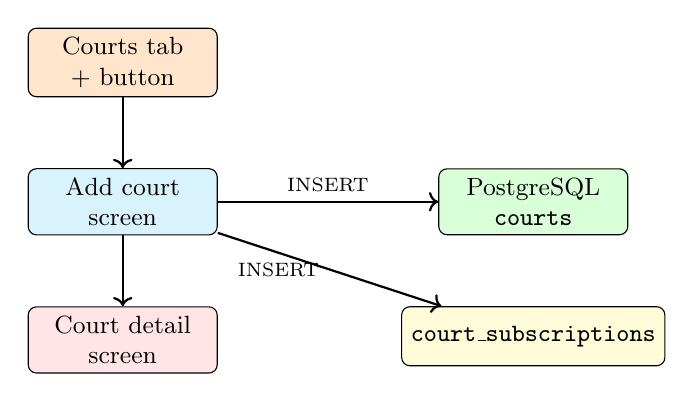
\begin{tikzpicture}[
  node distance=0.9cm,
  box/.style={rectangle, draw, rounded corners=3pt, minimum width=2.4cm, minimum height=0.75cm, align=center, font=\small},
  arr/.style={->, thick}
]
  \node[box, fill=orange!20] (tab) {Courts tab\\+ button};
  \node[box, fill=cyan!15, below=of tab] (add) {Add court\\screen};
  \node[box, fill=green!15, right=2.8cm of add] (db) {PostgreSQL\\\texttt{courts}};
  \node[box, fill=yellow!15, below=of db] (sub) {\texttt{court\_subscriptions}};
  \node[box, fill=red!10, below=of add] (detail) {Court detail\\screen};
  \draw[arr] (tab) -- (add);
  \draw[arr] (add) -- node[above, font=\scriptsize] {INSERT} (db);
  \draw[arr] (add) -- node[left, font=\scriptsize] {INSERT} (sub);
  \draw[arr] (add) -- (detail);
\end{tikzpicture}
\caption{Happy path: user opens Add court, saves, row is written, user is subscribed, app navigates to the new court.}
\end{figure}

%==============================================================================
\section{Concepts You Need (Minimal Background)}
%==============================================================================

\subsection{Latitude and Longitude}

A \textbf{coordinate pair} $(\text{lat}, \text{lng})$ pinpoints a point on Earth. The map component treats them as the truth for ``where is this court?'' Without them, you cannot place a marker reliably.

\textbf{Alternative:} only store an address string and geocode it on the server. RimRun still stores explicit numbers so the map works offline from cached data and avoids extra geocode API calls per add.

\subsection{Expo and React Native}

\textbf{Expo} wraps \textbf{React Native}: you write UI in JavaScript/TypeScript; it runs on iOS and Android. \texttt{expo-location} asks the OS for GPS permission and reads position. \texttt{react-native-maps} embeds the native map (Apple Maps on iOS, Google on Android).

\subsection{Supabase and the Anon Key}

The app uses the \textbf{public (anon) API key} plus the user's \textbf{JWT} (session token). PostgREST turns \texttt{.from('courts').insert(...)} into an HTTP request. \textbf{RLS} runs in Postgres \emph{before} the insert succeeds: if no policy allows the row, you get an error (often code \texttt{42501}).

\textbf{Alternative:} a custom backend (Node server) that validates input and inserts with a \textbf{service role} key. RimRun keeps inserts on the client for simplicity, and uses RLS to bound what users can do.

\subsection{Row Level Security (RLS) in One Sentence}

When RLS is \textbf{enabled} on \texttt{courts}, every row access checks \textbf{policies}. The migration adds: ``authenticated users may \texttt{SELECT} all courts'' and ``may \texttt{INSERT} only if \texttt{source = 'user'} and \texttt{created\_by} is the current user.''

%==============================================================================
\section{Where the Code Lives}
%==============================================================================

\begin{tabular}{@{}ll@{}}
\toprule
\textbf{Role} & \textbf{Path} \\
\midrule
Add-court UI & \texttt{app/(app)/court/add.tsx} \\
Entry from map & \texttt{app/(app)/(tabs)/courts.tsx} (\texttt{router.push("/(app)/court/add")}) \\
Stack route & \texttt{app/(app)/\_layout.tsx} registers \texttt{court/add} \\
SQL migration & \texttt{scripts/user-courts-migration.sql} \\
OSM import (contrast) & \texttt{scripts/import-courts.js} \\
\bottomrule
\end{tabular}

\subsection{Expo Router: Why \texttt{court/add.tsx} Matters}

Files under \texttt{app/} define URLs. A dynamic file \texttt{[courtId].tsx} matches \emph{any} segment, including the word \texttt{add}---which would wrongly open the \textbf{detail} screen for a fake id ``add.'' A \textbf{static} file \texttt{add.tsx} takes precedence, so \texttt{/court/add} is the form screen.

\textbf{Alternative:} use a query param or a different path like \texttt{court/new}. Static \texttt{add} is readable and avoids collision with \texttt{[courtId]}.

%==============================================================================
\section{Screen Layout: Map + Form}
%==============================================================================

\begin{figure}[h]
\centering
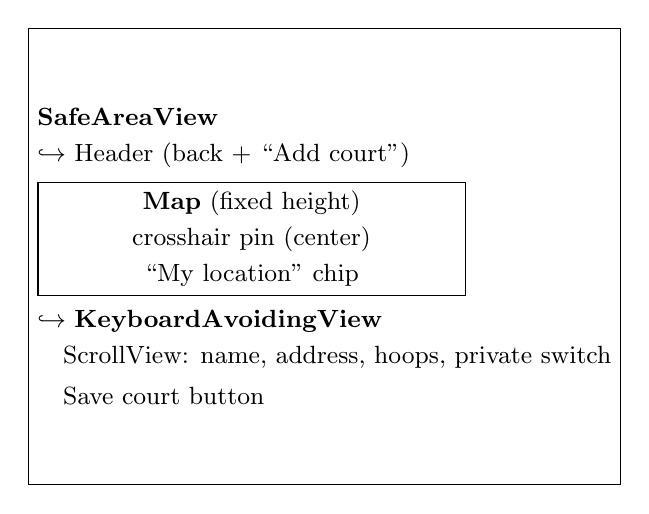
\begin{tikzpicture}[node distance=0.35cm]
  \node[draw, minimum width=6cm, minimum height=5.8cm, align=left, font=\small] (phone) {%
    \textbf{SafeAreaView}\\[2pt]
    $\hookrightarrow$ Header (back + ``Add court'')\\[4pt]
    \fbox{\parbox{5.2cm}{\centering\textbf{Map} (fixed height)\\[2pt]
    crosshair pin (center)\\[2pt]
    ``My location'' chip}}\\[4pt]
    $\hookrightarrow$ \textbf{KeyboardAvoidingView}\\[2pt]
    \quad ScrollView: name, address, hoops, private switch\\[4pt]
    \quad Save court button
  };
\end{tikzpicture}
\caption{Vertical structure: map occupies a fixed band; form scrolls beneath (important when the keyboard opens).}
\end{figure}

\subsection{Safe Area}

\texttt{SafeAreaView} with \texttt{edges=\{['top']\}} keeps the header below the notch/status bar. \textbf{Why not full edges?} The bottom tab bar already handles the home indicator region on many layouts; RimRun matches other stack screens (e.g.\ court detail).

\subsection{KeyboardAvoidingView}

On iOS, when the user focuses a \texttt{TextInput}, the keyboard slides up. \texttt{KeyboardAvoidingView} with \texttt{behavior="padding"} shrinks the inner layout so the submit button can stay reachable. Android often resizes the window automatically; behavior may be \texttt{undefined} there.

\textbf{Alternative:} \texttt{react-native-keyboard-aware-scroll-view}. The built-in approach keeps dependencies smaller.

%==============================================================================
\section{Choosing Coordinates: Crosshair + Map Region}
%==============================================================================

\subsection{What the Code Does}

\texttt{MapView} uses \texttt{initialRegion=\{region\}} once. When the user \textbf{pans or zooms}, \texttt{onRegionChangeComplete} updates React state \texttt{region}. The \textbf{visual pin} is not a map marker; it is a \textbf{fixed overlay} (Ionicon \texttt{location}) centered on the map view. So the geographic point being saved is always the \textbf{center of the visible map}.

\begin{figure}[h]
\centering
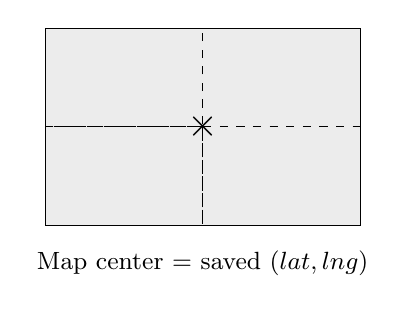
\begin{tikzpicture}
  \draw[fill=gray!15] (0,0) rectangle (4,2.5);
  \draw[dashed] (2,1.25) -- (2,0) -- (2,2.5);
  \draw[dashed] (2,1.25) -- (0,1.25) -- (4,1.25);
  \node at (2,1.25) {\Large$\times$};
  \node[font=\small, below] at (2,-0.2) {Map center = saved $(\text{lat}, \text{lng})$};
\end{tikzpicture}
\caption{Crosshair pattern: the saved coordinates are the map's center after the user pans/zooms.}
\end{figure}

\subsection{Why Crosshair Instead of a Draggable Marker?}

A \textbf{draggable marker} is intuitive but easy to get wrong when combined with \texttt{onRegionChangeComplete}: both can update coordinates and \textbf{fight each other} (marker moved, then region callback snaps the pin). A crosshair has \textbf{one source of truth}: the region's \texttt{latitude}/\texttt{longitude}.

\textbf{Alternative:} tap on map to drop a pin (\texttt{onPress}). Good UX; slightly more code. Crosshair + pan is standard for ``move map under fixed pin.''

\subsection{Why Not \texttt{region=\{region\}} (Fully Controlled Map)?}

Fully controlling \texttt{region} from React re-renders the map on every update and can cause \textbf{jitter} or interrupt gestures. Using \texttt{initialRegion} + \texttt{onRegionChangeComplete} lets the native map own gesture state between commits.

\subsection{\texttt{My Location} Button}

\texttt{mapRef.current?.animateToRegion(next, 250)} moves the map so the user's GPS position becomes the center (and \texttt{onRegionChangeComplete} updates state). \textbf{Why animate?} Jumping the map without animation is disorienting.

\texttt{ZOOM\_DELTA = 0.008} sets how ``zoomed in'' the map is (degrees of span). Smaller delta = closer zoom.

\subsection{Default When GPS Fails or Permission Denied}

If permission is denied or \texttt{getCurrentPositionAsync} throws, RimRun falls back to a default region (San Francisco area). \textbf{Why?} The screen still loads; the user can pan to the real location. \textbf{Alternative:} block the screen until permission is granted---stricter but worse for first-time users exploring the app.

%==============================================================================
\section{Location Permissions}
%==============================================================================

\texttt{Location.requestForegroundPermissionsAsync()} is called on mount. \textbf{Foreground} means ``while the app is visible''---appropriate for placing a pin, not for background tracking.

\textbf{Why request again in \texttt{useMyLocation}?} The user may deny first, then open Settings and return; the chip re-requests before reading position.

%==============================================================================
\section{Form Fields and Validation}
%==============================================================================

\begin{description}[style=nextline, leftmargin=1.2cm]
    \item[Court name (required)] Trimmed; empty shows an alert. This is the minimum viable identity for list/map callouts.
    \item[Address (optional)] Free text; helps humans, not required for geometry.
    \item[Hoops (optional)] \texttt{parseHoops}: empty $\to$ \texttt{null}; otherwise integer clamped to $[0,10]$ (same spirit as \texttt{import-courts.js}). Invalid non-numeric input with non-empty string $\to$ alert.
    \item[Private switch] Maps to boolean \texttt{is\_private} for UI and filters (e.g.\ ``Private court'' on detail).
\end{description}

\textbf{Why clamp hoops?} Prevents nonsense values and matches import script conventions.

%==============================================================================
\section{The Row Inserted into \texttt{courts}}
%==============================================================================

The app sends a JSON object aligned with \textbf{bulk OSM imports} so one table holds both sources:

\begin{lstlisting}[language=Java]
{
  name, address, latitude, longitude, hoops, is_private,
  osm_id: null, osm_type: null,
  source: "user",
  confidence: 0.85,
  created_by: user.id,
}
\end{lstlisting}

\begin{itemize}[noitemsep]
    \item \texttt{osm\_id / osm\_type} are \texttt{null} for user courts. SQL unique constraint on \texttt{osm\_id} allows multiple NULLs (see \texttt{scripts/add-osm-unique.sql}).
    \item \texttt{source: "user"} distinguishes from \texttt{osm} rows for RLS (\texttt{WITH CHECK (source = 'user')}).
    \item \texttt{confidence: 0.85} is slightly below typical import \texttt{1.0}---a soft signal that user data may need moderation later.
    \item \texttt{created\_by} ties the row to \texttt{auth.users}; profile ``Courts added'' counts \texttt{WHERE created\_by = me}.
\end{itemize}

\textbf{Alternative:} separate table \texttt{user\_courts}. RimRun reuses \texttt{courts} so map queries stay simple (\texttt{SELECT * FROM courts}).

%==============================================================================
\section{After Insert: Subscription + Navigation}
%==============================================================================

\begin{enumerate}[noitemsep]
    \item \texttt{.insert(row).select('id').single()} returns the new UUID.
    \item \texttt{court\_subscriptions} insert: user is immediately ``following'' the court (chat, heart icon, Chats tab).
    \item \texttt{router.replace(\{ pathname: '/(app)/court/[courtId]', params: \{ courtId \} \})} opens detail without stacking Add court in history (back from detail goes to the previous screen, not the form).
\end{enumerate}

\textbf{Why \texttt{replace} not \texttt{push}?} Avoids an infinite-looking stack Add $\to$ Detail $\to$ back $\to$ Add.

\textbf{Alternative:} skip auto-subscribe; user must tap Subscribe on detail. Auto-subscribe matches the expectation ``I just created this court.''

%==============================================================================
\section{Database Migration: \texttt{user-courts-migration.sql}}
%==============================================================================

Without this script, the app uses the anon key: either \texttt{created\_by} column is missing (insert error) or RLS blocks inserts.

\begin{figure}[h]
\centering
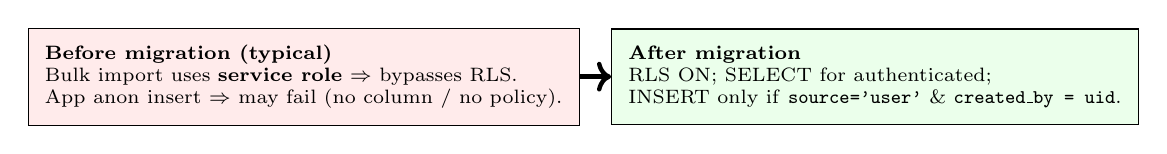
\begin{tikzpicture}[
  box/.style={rectangle, draw, align=left, font=\scriptsize, inner sep=6pt}
]
  \node[box, fill=red!8] (before) {\textbf{Before migration (typical)}\\Bulk import uses \textbf{service role} $\Rightarrow$ bypasses RLS.\\App anon insert $\Rightarrow$ may fail (no column / no policy).};
  \node[box, fill=green!8, right=0.4cm of before] (after) {\textbf{After migration}\\RLS ON; SELECT for authenticated;\\INSERT only if \texttt{source='user'} \& \texttt{created\_by = uid}.};
  \draw[->, ultra thick] (before) -- (after);
\end{tikzpicture}
\caption{Service role scripts are all-powerful; the mobile app is intentionally limited.}
\end{figure}

\subsection{Why \texttt{created\_by = auth.uid()} in Policy, Not Just in App?}

The client \emph{could} lie if the server only trusted the JSON body. Postgres \texttt{WITH CHECK (created\_by = auth.uid())} forces the stored value to match the session. (A malicious client could still set \texttt{source}; the policy ties \texttt{created\_by} to the real user.)

\textbf{Note:} \texttt{source = 'user'} is also checked---stops inserting rows that pretend to be OSM from the app.

\subsection{Why \texttt{SELECT} Policy \texttt{using (true)} for Authenticated?}

Every logged-in user can read all courts so the \textbf{map} can load pins in one query. \textbf{Tighter alternative:} hide courts until approved (moderation queue)---not implemented yet.

\subsection{\texttt{ON DELETE SET NULL} on \texttt{created\_by}}

If an auth user is deleted, the court row can remain (community asset) while losing creator linkage.

%==============================================================================
\section{Error Handling in the App}
%==============================================================================

If the error message suggests RLS or code \texttt{42501}, the alert tells the developer to run \texttt{user-courts-migration.sql}. Other errors surface the raw message for debugging.

%==============================================================================
\section{Summary: Design Choices vs Alternatives}
%==============================================================================

\begin{tabular}{@{}p{3.2cm}p{4.5cm}p{4.8cm}@{}}
\toprule
\textbf{Topic} & \textbf{RimRun choice} & \textbf{Common alternative} \\
\midrule
Coordinates & Map center + crosshair state & Draggable marker; address-only + geocode \\
Map control & \texttt{initialRegion} + callbacks & Fully controlled \texttt{region} prop \\
Save target & Single \texttt{courts} table & Separate user-submission table \\
Security & RLS + \texttt{created\_by} check & Edge Function + service role \\
After save & Auto-subscribe + \texttt{replace} & Manual subscribe; \texttt{push} stack \\
Source tag & \texttt{source: "user"} & No distinction; trust all inserts \\
\bottomrule
\end{tabular}

%==============================================================================
\section{Checklist: Making It Work End-to-End}
%==============================================================================

\begin{enumerate}[noitemsep]
    \item \texttt{public.courts} exists with columns compatible with the insert (lat/lng, name, etc.).
    \item Run \texttt{scripts/user-courts-migration.sql} in Supabase SQL Editor.
    \item User is logged in (JWT present on Supabase client).
    \item Location permission granted for best UX (optional: pan from default region).
\end{enumerate}

\end{document}
